\documentclass[problem]{mcs}

\begin{pcomments}
  \pcomment{spring07 pset4-6}
  \pcomment{PS_graph_maximal_connected}
\end{pcomments}

\pkeywords{
 graph theory
 connected_component
 components 
}


\begin{problem}
A set, $M$, of vertices of a graph is a \emph{maximal connected} set if
every pair of vertices in the set are connected, and any set of vertices
properly containing $M$ will contain two vertices that are not connected.

\bparts

\ppart What are the maximal connected subsets of the following
(unconnected) graph?
\begin{figure}[h]\redrawn
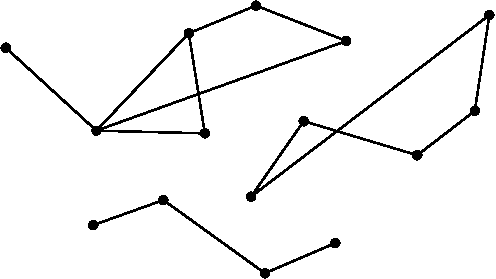
\includegraphics{3comp}
\end{figure}
\begin{solution} 
There are three maximal subsets, each one equal to the vertices of one of
the connected components of the graph.
\end{solution}

\ppart Explain the connection between maximal connected sets and connected
components.  Prove it.

\begin{solution} 
They are the same.

We first show that a connected component is a maximal set.  A connected
component consists of \emph{all} the vertices connected to some vertex
$v$.  A larger set of vertices would, by definition, contain both $v$ and
a vertex, $w$, that is not in the connected component.  This means that
$w$ is not connected to $v$, and therefore the larger set is not
connected.  So a connected component is maximal.

Conversely, suppose we have a maximal connected set, $M$.  Since $M$ is
connected, any vertex, $v$, in $M$ is connected to all the other vertices
in $M$.  If there was any vertex, $w$, connected to $v$, that was not in
$M$, then $M \union \set{w}$ would be connected and properly contain $M$,
contradicting the maximality of $M$.  So $M$ consists of exactly the
vertices connected to $v$, proving that it is a connected component.
\end{solution}

\eparts
\end{problem}

